\section{Implementación de motor a paso.}

\begin{frame}{Librería de stepperMotor}
    \begin{columns}[c]
        \column{0.5\textwidth}{
        \begin{figure}[H]
            \centering
            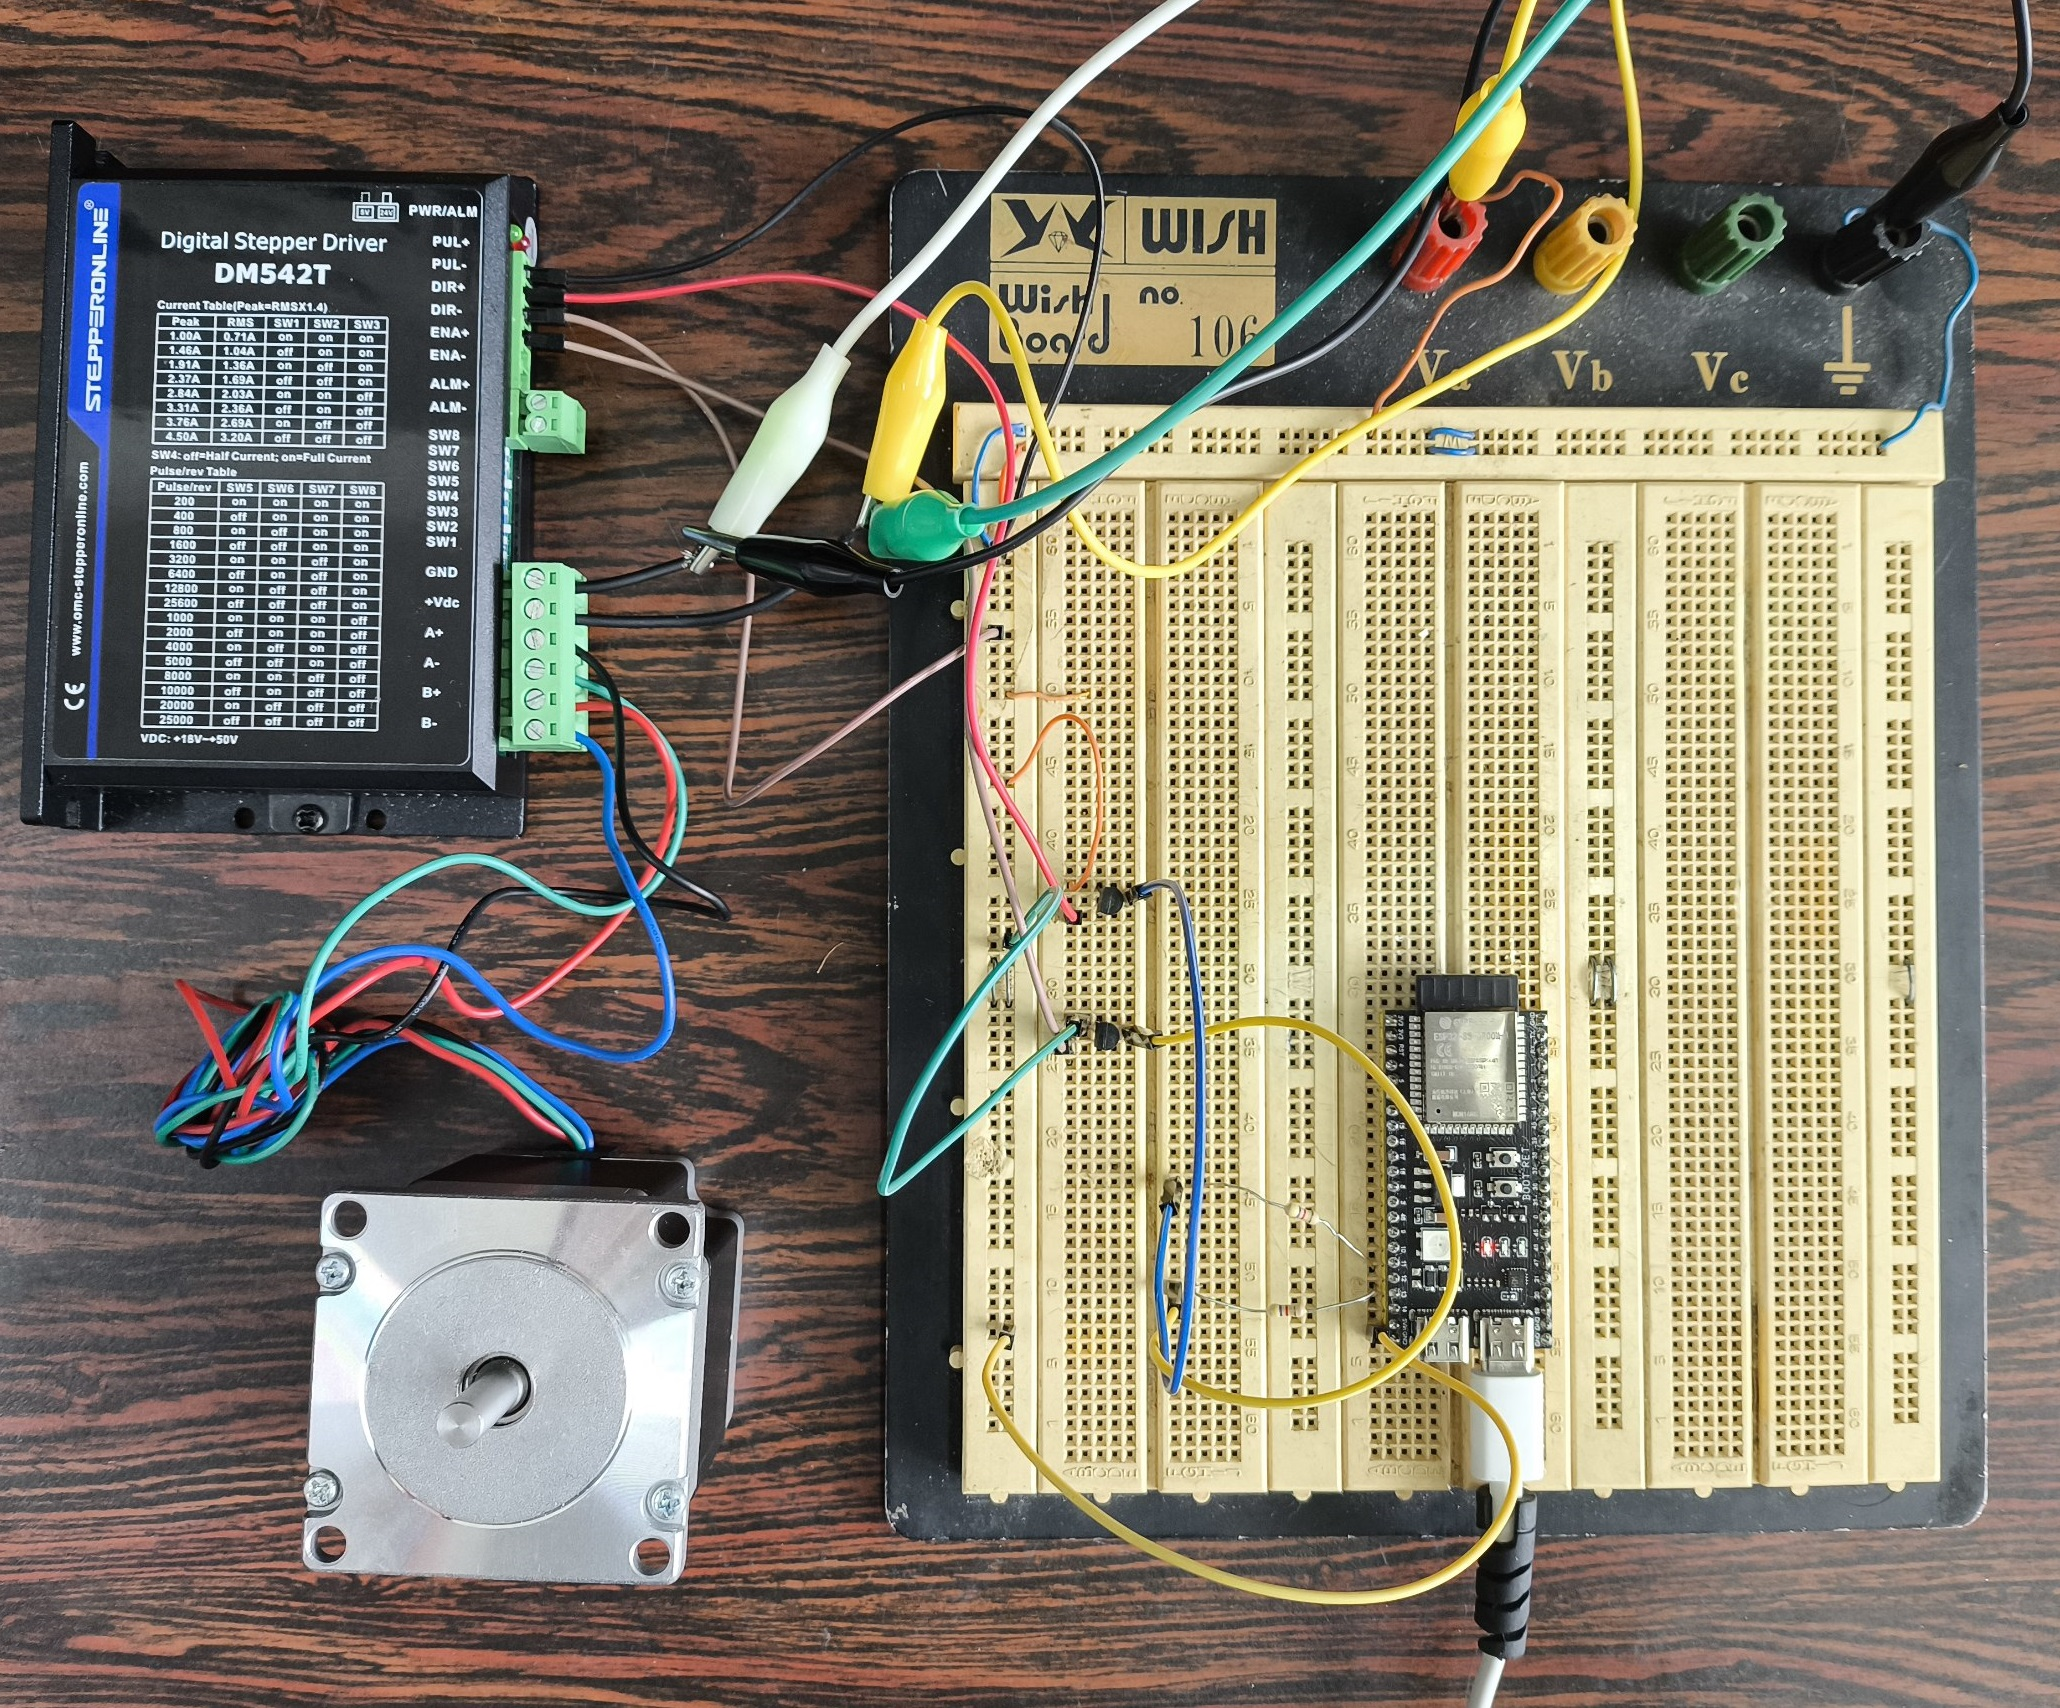
\includegraphics[width=\textwidth]{fig/motor-esp.jpg}
            \caption{Diagrama de conexiones driver y motor, en conjunto con el ESP32.}
        \end{figure}
        }

        \column{0.5\textwidth}{
            \begin{exampleblock}{Fórmula General:}
                \begin{equation}\label{eq:f}
                    \frac{f_{pulsos}}{f_{motor}} = PPR
                \end{equation}
            \end{exampleblock}
            \begin{itemize}
                \item $f_{pulsos}$: Frecuencia de pulsos enviada al driver por PUL (Hz).
                \item $f_{motor}$: Frecuencia de rotación del motor (Hz) (RPM/60).
                \item $PPR$: Pulsos por revolución del motor que depende del driver.
            \end{itemize}          
        }
    \end{columns}  
\end{frame}